\documentclass{standalone}
\usepackage{tikz}
\usetikzlibrary{patterns, positioning}
\usetikzlibrary{shapes.misc}
\usepackage[outline]{contour}
\contourlength{1.5pt} 


\begin{document}
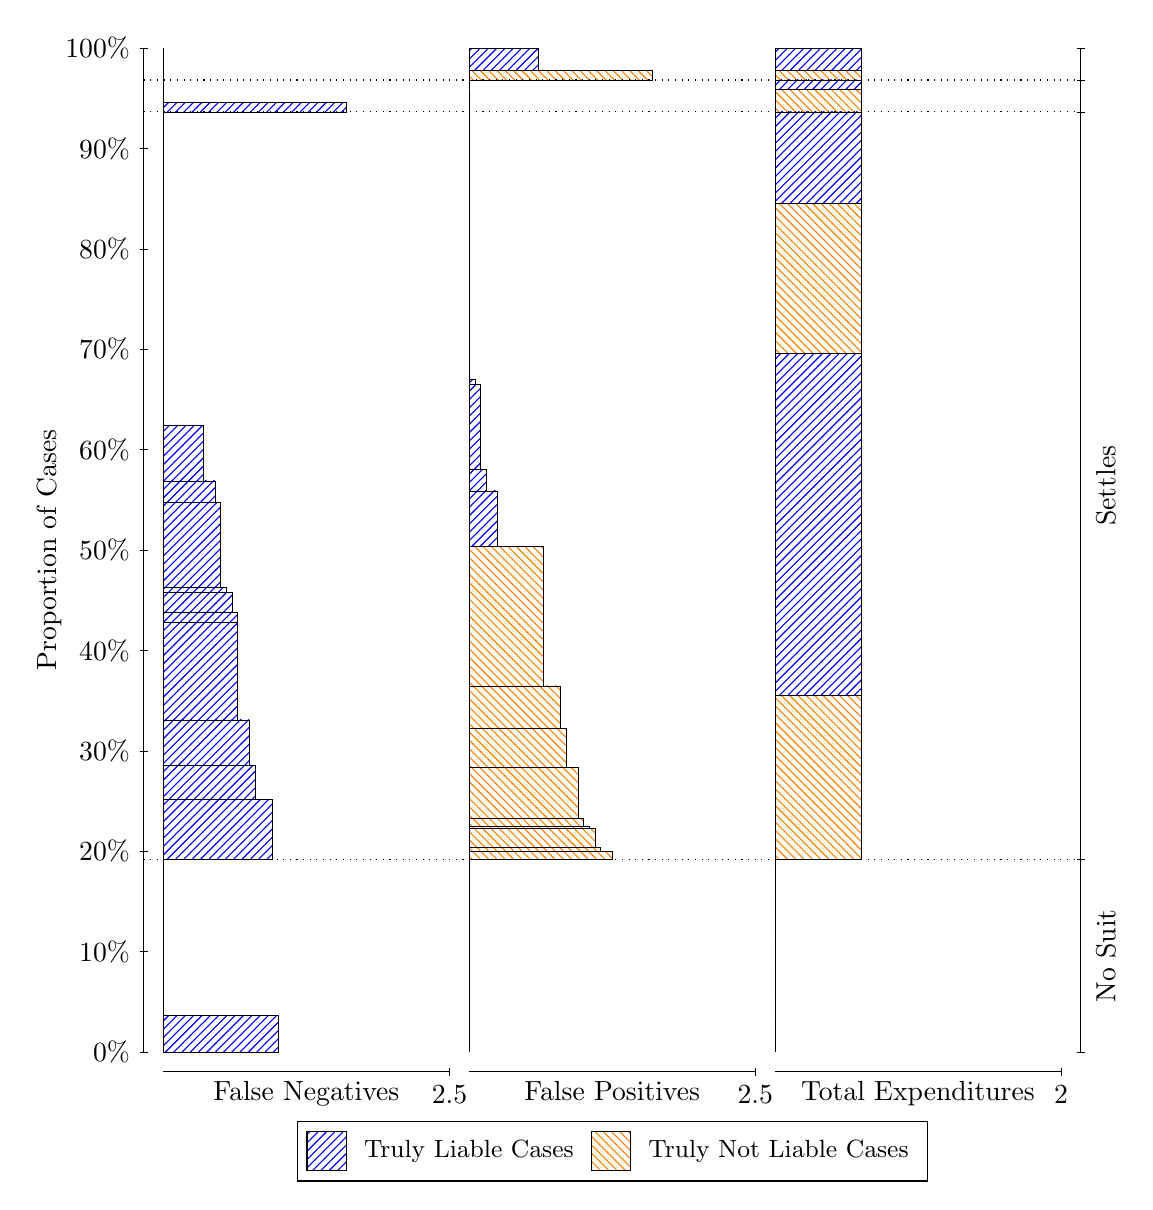
\begin{tikzpicture}
\draw[black, very thin] (1.5,1.75) -- (1.5,14.5);
\node[rotate=90, text=black, anchor=center] at (0.3, 8.125) {Proportion of Cases};
\draw[black, very thin] (1.45,1.75) -- (1.55,1.75);
\node[text=black, anchor=east] at (1.45, 1.75) {0\%};
\draw[black, very thin] (1.45,3.025) -- (1.55,3.025);
\node[text=black, anchor=east] at (1.45, 3.025) {10\%};
\draw[black, very thin] (1.45,4.3) -- (1.55,4.3);
\node[text=black, anchor=east] at (1.45, 4.3) {20\%};
\draw[black, very thin] (1.45,5.575) -- (1.55,5.575);
\node[text=black, anchor=east] at (1.45, 5.575) {30\%};
\draw[black, very thin] (1.45,6.85) -- (1.55,6.85);
\node[text=black, anchor=east] at (1.45, 6.85) {40\%};
\draw[black, very thin] (1.45,8.125) -- (1.55,8.125);
\node[text=black, anchor=east] at (1.45, 8.125) {50\%};
\draw[black, very thin] (1.45,9.4) -- (1.55,9.4);
\node[text=black, anchor=east] at (1.45, 9.4) {60\%};
\draw[black, very thin] (1.45,10.675) -- (1.55,10.675);
\node[text=black, anchor=east] at (1.45, 10.675) {70\%};
\draw[black, very thin] (1.45,11.95) -- (1.55,11.95);
\node[text=black, anchor=east] at (1.45, 11.95) {80\%};
\draw[black, very thin] (1.45,13.225) -- (1.55,13.225);
\node[text=black, anchor=east] at (1.45, 13.225) {90\%};
\draw[black, very thin] (1.45,14.5) -- (1.55,14.5);
\node[text=black, anchor=east] at (1.45, 14.5) {100\%};

\draw[black, very thin] (13.4,1.75) -- (13.4,14.5);
\draw[black, very thin] (13.35,1.75) -- (13.45,1.75);
\node[anchor=west] at (13.35, 1.75) {};
\draw[black, very thin] (13.35,4.1919) -- (13.45,4.1919);
\node[anchor=west] at (13.35, 4.1919) {};
\draw[black, very thin] (13.35,13.689) -- (13.45,13.689);
\node[anchor=west] at (13.35, 13.689) {};
\draw[black, very thin] (13.35,14.094) -- (13.45,14.094);
\node[anchor=west] at (13.35, 14.094) {};
\draw[black, very thin] (13.35,14.5) -- (13.45,14.5);
\node[anchor=west] at (13.35, 14.5) {};

\draw[black, very thin, pattern color=blue, pattern=north east lines] (1.75,1.75) rectangle (3.2033,2.2108);
\draw[black, very thin, pattern color=orange, pattern=north west lines] (1.75,2.2108) rectangle (1.75,4.1919);
\draw[black, very thin, pattern color=blue, pattern=north east lines] (1.75,4.1919) rectangle (3.1307,4.9543);
\draw[black, very thin, pattern color=blue, pattern=north east lines] (1.75,4.9543) rectangle (2.9127,5.3941);
\draw[black, very thin, pattern color=blue, pattern=north east lines] (1.75,5.3941) rectangle (2.84,5.9689);
\draw[black, very thin, pattern color=blue, pattern=north east lines] (1.75,5.9689) rectangle (2.6947,7.2035);
\draw[black, very thin, pattern color=blue, pattern=north east lines] (1.75,7.2035) rectangle (2.6947,7.3289);
\draw[black, very thin, pattern color=blue, pattern=north east lines] (1.75,7.3289) rectangle (2.622,7.5896);
\draw[black, very thin, pattern color=blue, pattern=north east lines] (1.75,7.5896) rectangle (2.5493,7.648);
\draw[black, very thin, pattern color=blue, pattern=north east lines] (1.75,7.648) rectangle (2.4767,8.7269);
\draw[black, very thin, pattern color=blue, pattern=north east lines] (1.75,8.7269) rectangle (2.404,9.0039);
\draw[black, very thin, pattern color=blue, pattern=north east lines] (1.75,9.0039) rectangle (2.2587,9.7057);
\draw[black, very thin, pattern color=orange, pattern=north west lines] (1.75,9.7057) rectangle (1.75,13.689);
\draw[black, very thin, pattern color=blue, pattern=north east lines] (1.75,13.689) rectangle (4.0753,13.809);
\draw[black, very thin, pattern color=orange, pattern=north west lines] (1.75,13.809) rectangle (1.75,14.094);
\draw[black, very thin, pattern color=orange, pattern=north west lines] (1.75,14.094) rectangle (1.75,14.22);
\draw[black, very thin, pattern color=blue, pattern=north east lines] (1.75,14.22) rectangle (1.75,14.5);
\draw[black, very thin, pattern color=orange, pattern=north west lines] (5.6333,1.75) rectangle (5.6333,3.7311);
\draw[black, very thin, pattern color=blue, pattern=north east lines] (5.6333,3.7311) rectangle (5.6333,4.1919);
\draw[black, very thin, pattern color=orange, pattern=north west lines] (5.6333,4.1919) rectangle (7.45,4.2976);
\draw[black, very thin, pattern color=orange, pattern=north west lines] (5.6333,4.2976) rectangle (7.3047,4.3504);
\draw[black, very thin, pattern color=orange, pattern=north west lines] (5.6333,4.3504) rectangle (7.232,4.5938);
\draw[black, very thin, pattern color=orange, pattern=north west lines] (5.6333,4.5938) rectangle (7.1593,4.6133);
\draw[black, very thin, pattern color=orange, pattern=north west lines] (5.6333,4.6133) rectangle (7.0867,4.718);
\draw[black, very thin, pattern color=orange, pattern=north west lines] (5.6333,4.718) rectangle (7.014,5.3673);
\draw[black, very thin, pattern color=orange, pattern=north west lines] (5.6333,5.3673) rectangle (6.8687,5.8595);
\draw[black, very thin, pattern color=orange, pattern=north west lines] (5.6333,5.8595) rectangle (6.796,6.398);
\draw[black, very thin, pattern color=orange, pattern=north west lines] (5.6333,6.398) rectangle (6.578,8.1749);
\draw[black, very thin, pattern color=blue, pattern=north east lines] (5.6333,8.1749) rectangle (5.9967,8.8767);
\draw[black, very thin, pattern color=blue, pattern=north east lines] (5.6333,8.8767) rectangle (5.8513,9.1536);
\draw[black, very thin, pattern color=blue, pattern=north east lines] (5.6333,9.1536) rectangle (5.7787,10.233);
\draw[black, very thin, pattern color=blue, pattern=north east lines] (5.6333,10.233) rectangle (5.706,10.291);
\draw[black, very thin, pattern color=blue, pattern=north east lines] (5.6333,10.291) rectangle (5.6333,13.689);
\draw[black, very thin, pattern color=orange, pattern=north west lines] (5.6333,13.689) rectangle (5.6333,13.974);
\draw[black, very thin, pattern color=blue, pattern=north east lines] (5.6333,13.974) rectangle (5.6333,14.094);
\draw[black, very thin, pattern color=orange, pattern=north west lines] (5.6333,14.094) rectangle (7.9587,14.22);
\draw[black, very thin, pattern color=blue, pattern=north east lines] (5.6333,14.22) rectangle (6.5053,14.5);
\draw[black, very thin, pattern color=orange, pattern=north west lines] (9.5167,1.75) rectangle (9.5167,3.7311);
\draw[black, very thin, pattern color=blue, pattern=north east lines] (9.5167,3.7311) rectangle (9.5167,4.1919);
\draw[black, very thin, pattern color=orange, pattern=north west lines] (9.5167,4.1919) rectangle (10.607,6.2756);
\draw[black, very thin, pattern color=blue, pattern=north east lines] (9.5167,6.2756) rectangle (10.607,10.625);
\draw[black, very thin, pattern color=orange, pattern=north west lines] (9.5167,10.625) rectangle (10.607,12.524);
\draw[black, very thin, pattern color=blue, pattern=north east lines] (9.5167,12.524) rectangle (10.607,13.689);
\draw[black, very thin, pattern color=orange, pattern=north west lines] (9.5167,13.689) rectangle (10.607,13.974);
\draw[black, very thin, pattern color=blue, pattern=north east lines] (9.5167,13.974) rectangle (10.607,14.094);
\draw[black, very thin, pattern color=orange, pattern=north west lines] (9.5167,14.094) rectangle (10.607,14.22);
\draw[black, very thin, pattern color=blue, pattern=north east lines] (9.5167,14.22) rectangle (10.607,14.5);
\draw[black, dotted] (1.5,4.1919) -- (13.4,4.1919);
\draw[black, dotted] (1.5,13.689) -- (13.4,13.689);
\draw[black, dotted] (1.5,14.094) -- (13.4,14.094);
\draw[black, very thin] (1.75,1.5) -- (5.3833,1.5);
\node[text=black, anchor=north] at (3.5667, 1.5) {False Negatives};
\draw[black, very thin] (5.3833,1.45) -- (5.3833,1.55);
\node[text=black, anchor=north] at (5.3833, 1.45) {2.5};

\draw[black, very thin] (5.6333,1.5) -- (9.2667,1.5);
\node[text=black, anchor=north] at (7.45, 1.5) {False Positives};
\draw[black, very thin] (9.2667,1.45) -- (9.2667,1.55);
\node[text=black, anchor=north] at (9.2667, 1.45) {2.5};

\draw[black, very thin] (9.5167,1.5) -- (13.15,1.5);
\node[text=black, anchor=north] at (11.333, 1.5) {Total Expenditures};
\draw[black, very thin] (13.15,1.45) -- (13.15,1.55);
\node[text=black, anchor=north] at (13.15, 1.45) {2};

\node[text=black, centered, rotate=90] at (13.72, 2.9709) {\contour{white}{No Suit}};
\node[text=black, centered, rotate=90] at (13.72, 8.9403) {\contour{white}{Settles}};



\draw (7.449999999999999,1.5) node[draw=none] (baseCoordinate) {};
\begin{scope}[align=center]
        \matrix[scale=0.5, draw=black, below=0.5cm of baseCoordinate, nodes={draw}, column sep=0.1cm]{
            \node[rectangle, draw, minimum width=0.5cm, minimum height=0.5cm, pattern color=blue, pattern=north east lines] {}; &
            \node[draw=none, font=\small, text=black] (B) {Truly Liable Cases}; &
            \node[rectangle, draw, minimum width=0.5cm, minimum height=0.5cm, pattern color=orange, pattern=north west lines] {}; &
            \node[draw=none, font=\small, text=black] (B) {Truly Not Liable Cases}; \\
            };
\end{scope}

\end{tikzpicture}
\end{document}